\chapter{Priors for Gaussians}


\section{The Wishart or alternatively Inverse-Wishart distribution}

See Steven Nydick's ``The Wihart and Inverse Wishart Distributions''
on the web. This is the multi-dimensional generalisation of the Gamma
distribution. It is the conjugate prior to use for the precision matrix
of the MVG. I am currently still unsure which one to implement (if
not both). Factors to consider is how commonly they appear and how
well they will blend with the rest of the system. The Wishart version
corresponds to a multi-variate Gamma or Chi-Squared which gives it
a very generic standing. On the other hand, we may be able to do a
sigma-point type of thing with the Inverse Wishart fractionally easier.
We might also want to consider the triangular form. However, in the
end it seems that they are pretty much two versions of the same thing.
\begin{itemize}
\item I am not sure if we will use this on its own, apart from a building
block in the Gaussian-Wishart. Which, of course, is enough reason
to build this.
\item Check its relationship to the exponential family.
\item Check wether it has a canonical form that will support our required
set of factor operations.
\item What about a triangular form?
\item Check if we can develop a sigma-point form for this that we can easily
convert (both ways) between Wishart and a carefully selected set of
samples from it. Each sigma point will then comprise a full precision/covariance
matrix.
\end{itemize}

\subsection{Gamma distribution for the scalar case}

Lets consider IID scalar Gaussian RVs $X_{n}\sim\mathcal{N}(0,\sigma_{X}^{2})$.
We use standard theory on transforming random variables to find the
distribution of $Y_{n}=X_{n}^{2}$ as:

\begin{align*}
p(y_{n}|a=\frac{1}{2},b=\frac{1}{2\sigma_{X}^{2}}) & \propto y_{n}^{\frac{1}{2}-1}e^{-\frac{1}{2\sigma_{X}^{2}}y_{n}}.
\end{align*}


We recognise this as a Gamma distribution with characteristic function:

\begin{align*}
\Phi_{Y_{n}}(\omega) & =\left(\frac{\frac{1}{2\sigma_{X}^{2}}}{\frac{1}{2\sigma_{X}^{2}}-j\omega}\right)^{\frac{1}{2}}.
\end{align*}


Summing $N$ of these $Y_{i}$'s i.e. $Z=\sum_{n=1}^{N}X_{n}^{2}$
then has a a characteristic function:

\begin{align*}
\Phi_{Z}(\omega) & =\left(\frac{\frac{1}{2\sigma_{X}^{2}}}{\frac{1}{2\sigma_{X}^{2}}-j\omega}\right)^{\frac{N}{2}}.
\end{align*}


This is another Gamma distribution:

\begin{align*}
p(z|a=\frac{N}{2},b=\frac{1}{2\sigma_{X}^{2}}) & \propto z^{\frac{N}{2}-1}e^{-\frac{1}{2\sigma_{X}^{2}}z}.
\end{align*}


There are a number of distributions that match this general form as
is summarised in Table~\ref{tab:gamma_family}.

\begin{table}
\noindent \begin{centering}
$\begin{array}{cccccccc}
N & \sigma_{X}^{2} & a & b & p(z) & \Phi_{Z}(\omega) & \mathbb{E}[Z] & \text{var}(Z)\\
\hline 2a>0 & \frac{1}{2b}>0 & \frac{N}{2} & \frac{1}{2\sigma_{X}^{2}} & \text{Gam}(a,b) & \left(\frac{b}{b-j\omega}\right)^{a} & \frac{a}{b}=N\sigma_{X}^{2} & \frac{a}{b^{2}}=2N\sigma_{X}^{4}\\
2 & \frac{1}{2b}>0 & 1 & \frac{1}{2\sigma_{X}^{2}} & \text{Exp}(a) & \left(\frac{b}{b-j\omega}\right)^{1} & 2\sigma_{X}^{2} & 4\sigma_{X}^{4}\\
2,4,6\ldots & \frac{1}{2b}>0 & N'=\frac{N}{2} & \frac{1}{2\sigma_{X}^{2}} & \text{\ensuremath{\text{Erl}(b,N'=N/2)}} & \left(\frac{b}{b-j\omega}\right)^{N'} & 2N'\sigma_{X}^{2} & 4N'\sigma_{X}^{4}\\
1,2\ldots & 1 & \frac{N}{2} & \frac{1}{2} & \text{Chi}^{2}(N) & \left(\frac{\frac{1}{2}}{\frac{1}{2}-j\omega}\right)^{\frac{N}{2}} & N & 2N
\end{array}$
\par\end{centering}

\caption{Family of Gamma related distributions. Note that $\sigma_{X}^{2}$
is the variance of $X$, not of $Z$.}


\label{tab:gamma_family}
\end{table}


Bottom line for the most generic case: If we sum the squares of a
certain number (which also could be non-integer i.e. positive real-valued)
of iid zero-mean Gaussians, we end up with a Gamma distribution for
the sum. The $2b$ is the precision of the original $X$'s and $2a$
is the number of those $X$'s we squared and added.

How does this relate to the prior for the unknown variance of $X$
-- given by $\sigma_{x}^{2}=\mathbb{E}[X^{2}-(\mu_{X})^{2}]$? Lets
consider the likelihood function

\begin{align*}
p(x_{1\ldots N}|\mu_{X},\sigma_{X}^{2}) & =K\prod_{n=1}^{N}\lambda^{\frac{1}{2}}e^{-\frac{\lambda}{2}(x_{n}-\mu)^{2}}\\
 & \propto\lambda^{\frac{N}{2}}e^{-\frac{\lambda}{2}\sum_{n=1}^{N}(x_{n}-\mu)^{2}}
\end{align*}
with $x_{1\ldots N}$, $\mu_{X}$ known, and $\lambda_{X}=\frac{1}{\sigma_{X}^{2}}$
the unknown precision. The corresponding conjugate prior thus needs
a product of a power of $\lambda$ with the exponent of an expression
linear%
\footnote{If we worked with the variance instead of the precision we will no
longer have a linear expression in the exponent.%
} in $\lambda$ i.e. the Gamma distribution. We therefore use the Gamma
distribution:

\begin{align*}
p(\lambda|a_{0},b_{0}) & \propto\lambda^{a_{0}-1}e^{-\lambda b_{0}}
\end{align*}
 as prior for $\lambda$. We must specify a $b_{0}$ that is related
to our initial guess of the precision $\lambda_{0}=\frac{1}{\sigma_{0}^{2}}$.
For that we first choose an $a_{0}=\frac{N_{0}}{2}$ where $N_{0}$
is the assumed number of initial observations we based our $b_{0}$
on. Since $\mathbb{E}[\lambda]=\frac{a}{b}$ we set $\frac{1}{\sigma_{0}^{2}}=\frac{N_{0}}{2b_{0}}$
i.e. $b_{0}=\frac{N_{0}\sigma_{0}^{2}}{2}$. We multiply to get the
posterior:

\begin{align*}
p(\lambda|x_{1\ldots N},\mu_{X};a_{0},b_{0}) & \propto\lambda^{a_{0}+\frac{N}{2}-1}e^{-\lambda\left(b_{0}+\frac{1}{2}\sum_{n=1}^{N}(x_{n}-\mu)^{2}\right)}
\end{align*}


\textbf{Example:} Lets sample data from a zero-mean $X$ with true
variance 3 i.e. the true precision is $\frac{1}{3}$. We'll assume
$N_{0}=4$ prior samples (i.e. $a_{0}=2$) and 'guess' our initial
variance as $\sigma_{0}^{2}=1$ (i.e. $b_{0}=2)$. Then we'll proceed
to extract 33 samples from the actual distribution of $X$ and update
our estimate for the precision. Figure~\ref{fig:prec_prior_and_posterior_1d}
shows clearly how our prior 'guess' is refined by the subsequent observations.

\begin{figure}
\noindent \begin{centering}
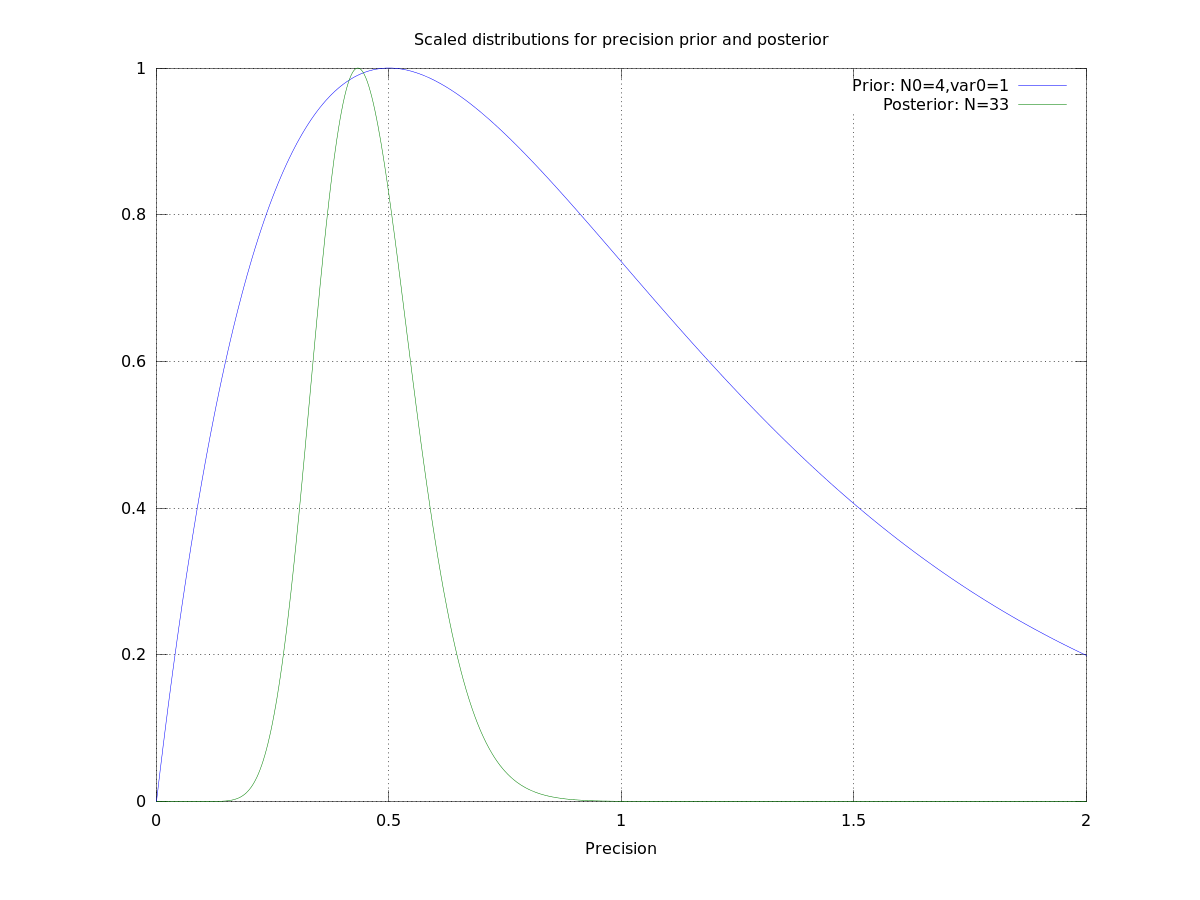
\includegraphics[height=5cm]{precision_prior_and_posterior_1d}
\par\end{centering}

\caption{Estimating the precision of a Gaussian: prior and posterior.}
\label{fig:prec_prior_and_posterior_1d}
\end{figure}


This is all very heart warming, but only applicable if $X$ is fully
observed. In the more general case we will need the full joint $p(X,\mu_{x},\Sigma_{X})$,
quite another kettle of fish.


\subsection{Wishart for the multi-variate case}

Since our RV is a matrix (instead of a vector), the covariance no
longer fits into a matrix, but now needs a 4-dimensional structure.


\section{The Gaussian-Wishart or alternatively Normal Inverse Wishart distribution}

The conjugate prior for the combined mean and precision/covariance
of the Gaussian distribution.


\subsection{Factor operations}
\begin{itemize}
\item Products/divisions with other Gaussians, Wisharts or Gaussian-Wisharts
seems to involve only the product/division of the Gaussian parts with
each other, and the Wishart parts with each other.
\item The marginal wrt $\mathbf{X}$ will be Gaussian, while the marginal
wrt both $\mathbf{\mu}$ and $\Sigma$ will be GW/NIW again, the only
two marginals I think we will need.
\item On the observation side we probably only need to bother with observing
$\mathbf{X}$, it seems unlikely that we will have a need for observing
$\mathbf{\mu}$ and $\Sigma$.
\item We probably can get along without damping.
\item I am still unsure about the normalisation. If the Gaussian part is
in canonical form it is inherently normalised. I suspect a similar
result will hold for the Wishart part.
\end{itemize}
See Murphy pg 125 and on for details. On the wish list for a fine
day.



From the Wiki page: ``The least informative, proper Wishart prior
is obtained by setting n = p.

The prior mean of $W_p(V, n)$ is $nV-1$. This implies that a good
choice for $V$ is $n\mathcal{S}_0$, where $\mathcal{S}_0$ is some
prior guess for the covariance matrix.''
